% -*- coding: utf-8; -*-
% vim: set fileencoding=utf-8 :
\documentclass[english,submission]{programming}
%% First parameter: the language is 'english'.
%% Second parameter: use 'submission' for initial submission, remove it for camera-ready (see 5.1)

\usepackage{longtable,booktabs}
% Correct order of tables after \paragraph or \subparagraph
\usepackage{etoolbox}
\makeatletter
\patchcmd\longtable{\par}{\if@noskipsec\mbox{}\fi\par}{}{}
\makeatother
% Allow footnotes in longtable head/foot
\IfFileExists{footnotehyper.sty}{\usepackage{footnotehyper}}{\usepackage{footnote}}
\makesavenoteenv{longtable}

\usepackage[backend=biber]{biblatex}
\addbibresource{references.bib}

\providecommand{\tightlist}{%
  \setlength{\itemsep}{0pt}\setlength{\parskip}{0pt}}

\begin{document}

\title{Wildcard: End user modification of web applications through a
data table}
\subtitle{}% optional

\author{Geoffrey Litt}
\authorinfo{is bla bla bla}
\author{Daniel Jackson}
\authorinfo{is bla bla bla}
\affiliation{Massachusetts Institute of Technology}

\keywords{programming journal, paper formatting, submission preparation} % please provide 1--5 keywords


%%%%%%%%%%%%%%%%%%
%% These data MUST be filled for your submission. (see 5.3)
\paperdetails{
  %% perspective options are: art, sciencetheoretical, scienceempirical, engineering.
  %% Choose exactly the one that best describes this work. (see 2.1)
  perspective=art,
  %% State one or more areas, separated by a comma. (see 2.2)
  %% Please see list of areas in http://programming-journal.org/cfp/
  %% The list is open-ended, so use other areas if yours is/are not listed.
  area={Programming environments, Visual and live programming},
  %% You may choose the license for your paper (see 3.)
  %% License options include: cc-by (default), cc-by-nc
  % license=cc-by-sa,
}
%%%%%%%%%%%%%%%%%%

%%%%%%%%%%%%%%%%%%
%% These data are provided by the editors. May be left out on submission.
%\paperdetails{
%  submitted=2016-08-10,
%  published=2016-10-11,
%  year=2016,
%  volume=1,
%  issue=1,
%  articlenumber=1,
%}
%%%%%%%%%%%%%%%%%%

%%%%%%%%%%%%%%%%%%%%%%%%%%%%%
% Please go to https://dl.acm.org/ccs/ccs.cfm and generate your Classification
% System [view CCS TeX Code] stanz and copy _all of it_ to this place.
%% From HERE
\begin{CCSXML}
<ccs2012>
<concept>
<concept_id>10002944.10011122.10003459</concept_id>
<concept_desc>General and reference~Computing standards, RFCs and guidelines</concept_desc>
<concept_significance>300</concept_significance>
</concept>
<concept>
<concept_id>10010405.10010476.10010477</concept_id>
<concept_desc>Applied computing~Publishing</concept_desc>
<concept_significance>300</concept_significance>
</concept>
</ccs2012>
\end{CCSXML}

\ccsdesc[300]{General and reference~Computing standards, RFCs and guidelines}
\ccsdesc[500]{Applied computing~Publishing}

% To HERE
%%%%%%%%%%%%%%%%%%%%%%%

\maketitle

% Please always include the abstract.
% The abstract MUST be written according to the directives stated in 
% http://programming-journal.org/submission/
% Failure to adhere to the abstract directives may result in the paper
% being returned to the authors.
\begin{abstract}
Many people use Web applications that do not exactly meet their unique
needs. While the Web platform supports client-side modification through
user scripts and browser extensions, most people do not have the
programming skills to implement such modifications.

In this paper, we present a prototype of a browser extension called
Wildcard, that empowers users to casually tweak web applications without
programming. Wildcard shows the main data from a web page in a table,
and maintains a bidirectional connection between the table and the
original page. By directly manipulating the table, people can perform a
wide variety of modifications: sorting/filtering content, adding private
annotations, using spreadsheet formulas to fetch data from other web
services, using custom UI elements to edit form data, and more.

We present examples of using Wildcard to solve real world problems, and
explain the design principles behind the prototype. In the future, we
envision continuing to build Wildcard into a fully deployed system that
makes the web into a more malleable medium.
\end{abstract}


\hypertarget{introduction}{%
\section{Introduction}\label{introduction}}

In 2012, the travel site Airbnb removed the ability to sort listings by
price. Users could still filter down to a price range, but could no
longer view the cheapest listings first. Many users complained on online
message boards that the change seemed hostile to users. ``It's so
frustrating!..What is the logic behind not having this function?'' said
one user on the
\href{https://community.withairbnb.com/t5/Hosting/Sorting-listing-by-price/td-p/559404}{Airbnb
support forum}. Alas, the feature remains missing to this day.

This is a familiar situation in a world of web applications that are
frequently updated without user consent. For most people, when web
software does not quite meet their needs, their only recourse is to
complain to the developers and hope someone listens. If they know how to
program in Javascript, perhaps they can implement a user script or a
browser extension to patch the issue, but most people do not have these
programming skills. While many have become accustomed to this status
quo, we see it as a waste of the openness of the Web platform and the
general pliability of software. In \emph{Personal Dynamic Media}, Alan
Kay envisioned personal computing as a medium that let a user ``mold and
channel its power to his own needs,'' but today's software is far from
this vision.

In this paper, we introduce Wildcard\footnote{Wildcard was the internal
  pre-release name for Hypercard, which served as an inspiration for
  this project since it promoted software modification by end users and
  was a precursor to the modern Web.}, a browser extension that aims to
make software more malleable by enabling users to tweak web applications
without programming. Wildcard adds a panel to the bottom of a web page
that shows a structured table view of the main data in the page. The
table maintains a bidirectional connection to the original page---when
the user manipulates the table, the original page gets modified, and
vice versa.

In Wildcard, a user can sort Airbnb listings with just one intuitive
click on a table header, with no programming required. Beyond sorting
and filtering data, Wildcard also supports accessing third party APIs,
performing small computations, recording private user annotations, using
alternate UI widgets, and other useful changes. While Wildcard does not
support all changes someone might want to make to a website, it makes
broad subset of changes easily accessible to end users.

Under the hood, the implementation is straightforward, because a
programmer must manually write an adapter for each individual website,
which uses web scraping techniques to map the web page to the table.
\emph{todo: mention the other bits of extension code too} While
programming is required for part of the process, this is still very
different from traditional browser extensions---instead of the
programmer defining a narrow use case, the end user is able to make many
different changes on top of a single site-specific adapter. Programmers
can extend Wildcard with plugins which provide various bits of
functionality including connecting it to specific websites and web APIs,
but the end user never needs to do any traditional programming.

\emph{note the current prototype stage}

In this paper, we present examples of using Wildcard to solve real world
problems, and explain the design principles behind the prototype:

\emph{todo: bullet point the design principles here}

In the future, we envision building Wildcard into a fully deployed
system that makes the web into a more malleable medium. \emph{todo: this
needs something more}

\hypertarget{demos}{%
\section{Demos}\label{demos}}

To get a sense of how it feels to use Wildcard, let's see an example of
using it to help with booking a trip using the travel sites Airbnb and
Expedia.

\hypertarget{sorting-and-filtering}{%
\subsection{Sorting and filtering}\label{sorting-and-filtering}}

We start by opening up the Airbnb search listings page to look for a
place to stay. As mentioned before, this page annoyingly doesn't let us
sort by price, so we'll use Wildcard to fix that. First, we open up the
Wildcard panel, which shows a table corresponding to the search results
in the page. As we click around in the table, the corresponding row in
the page is highlighted so we can see the connection between the views.

To sort the page in ascending order by price, all we need to do is click
on a table header to sort the table, and the original page gets sorted
in the same order. We can also filter to only listings with a rating
above 4.5 using a filtering UI on the column header. (Filtering by
rating is another feature not offered in the Airbnb site.)

Note how after finishing the sorting and filtering, we can close the
table view and continue using the website in its original design. The
Wildcard interface is better for flexibly manipulating the underlying
data, but the original site will usually offer a more polished and
pleasant experience for viewing the data after it's in the desired form.

\hypertarget{row-actions}{%
\subsection{Row actions}\label{row-actions}}

Most websites that show tables of data also offer various actions that
can be taken on a row in the table, like adding an item to a shopping
cart. Wildcard has the ability to make these actions available in the
data table, passed through by the site-specific adapter. The main
advantage this provides to users is the ability to easily perform an
action in bulk across multiple rows.

For example, it's tedious on Airbnb to click on listings one by one to
add them to a list of favorites, or open the listings in a new tab.
Using Wildcard, we can just select multiple rows, right click, and then
choose an action from the context menu to apply to all the rows.

Within the site adapter, each action is implemented as a web automation
that can do anything available in Javascript running in the context of
the page: clicking on buttons in the UI, launching AJAX requests,
navigating to a new page, etc.

\hypertarget{user-annotations}{%
\subsection{User annotations}\label{user-annotations}}

It's often useful to annotate a web page with notes. Users can use
Wildcard to annotate a page by adding data into a new column, which is
then shown in context of the original page.

Here, we use this feature to jot down notes on pros and cons of various
listings:

When we come back later to the site, the annotations will still be
visible. To support this, the site adapter saves the user annotations to
browser local storage for persistence, and associates each table row
with a stable identifier from the original site.

\hypertarget{computation-with-formulas}{%
\subsection{Computation with formulas}\label{computation-with-formulas}}

The demos so far have shown small, straightforward tweaks that provide
useful conveniences while requiring very little effort. But Wildcard
also supports adding more sophisticated functionality through a formula
system.

When traveling without a car, it's nice to evaluate potential places to
stay based on how walkable the surroundings are. There's an online
service called Walkscore that can rate the walkability of any location
on a 1-100 scale. It would take way too much work to manually
cross-reference the scores with Airbnb locations, but we can use
Wildcard formulas to automatically integrate Walkscore values into the
page.

Wildcard includes a formula that uses the Walkscore API to fetch the
score for any latitude and longitude. When we call the formula, it
fetches the associated score and populates it into the page. By copy
pasting the formula into all the rows on the page, we can add Walkscore
data to all the search listings:

Programmers can extend Wildcard with new formulas, which are just
Javascript functions that take table data as input and return new data.
Formulas can access external APIs to fetch data, but cannot have side
effects that directly manipulate the page. Instead, they return data,
which the user can choose to add into the page by showing a column of
data in the page.

\emph{todo: demo of composing formulas (requires a real formula
system\ldots)}

\hypertarget{custom-ui-elements}{%
\subsection{Custom UI elements}\label{custom-ui-elements}}

It might seem that Wildcard is only useful on websites that display
lists of tabular data like search results. But in fact, the table
metaphor is flexible enough to represent many types of data. For
example, a flight search form on Expedia.com can be represented as a
table with a single row:

This alone doesn't provide additional value on top of the original form,
but it becomes useful when combined with two other features of Wildcard.
First, Wildcard offers writable cells, where edits in either the table
or the original site propagate in both directions. Second, Wildcard
offers UI widgets that allow users to graphically edit the value of a
cell.

Here's an example of using those features to help with filling in a
form. When filling in dates for a flight search, it's important to
correctly remember the planned dates for the trip. This often requires
opening up a separate calendar application to look up the dates, and
manually entering the dates into the form. In Wildcard, we can do this
without manual copying, by editing the date cell directly using a
datepicker widget that has access to our calendar information. Notice
how the dates in the original form update when we update the table
cells.

Custom UIs enable people to use a consistent UI to enter common types of
data across the web. They also allow a user to access their own private
data as part of a web interface, without needing to expose that private
data to the website.

The PDF version of the output will go here.

Probably make one giant full-page figure that explains the whole thing?

For example, in Fig.~\ref{fig:table} we open up a table view that
corresponds to search results on the Airbnb travel site.

\begin{figure}
\hypertarget{fig:table}{%
\centering
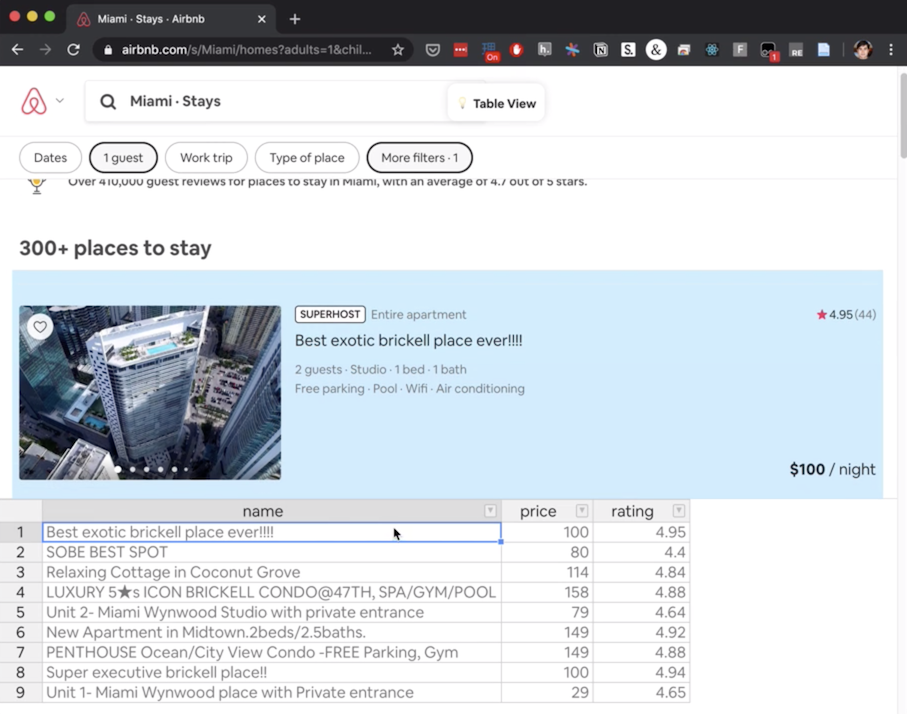
\includegraphics{media/opentable.png}
\caption{Opening a table corresponding to search results on
Airbnb}\label{fig:table}
}
\end{figure}

Overall, we think an interactive data table is a natural computation
model that presents a surprisingly large range of possibilities for end
user modification of websites. While we've presented just a small
sampling of use cases here to concretely illustrate some of these
possibilities, we plan to continue developing site adapters, formulas,
and UI elements to explore more use cases, and to eventually publicly
release the tool to allow real end users to discover their own uses.

\hypertarget{system-architecture}{%
\section{System Architecture}\label{system-architecture}}

\begin{figure}
\centering
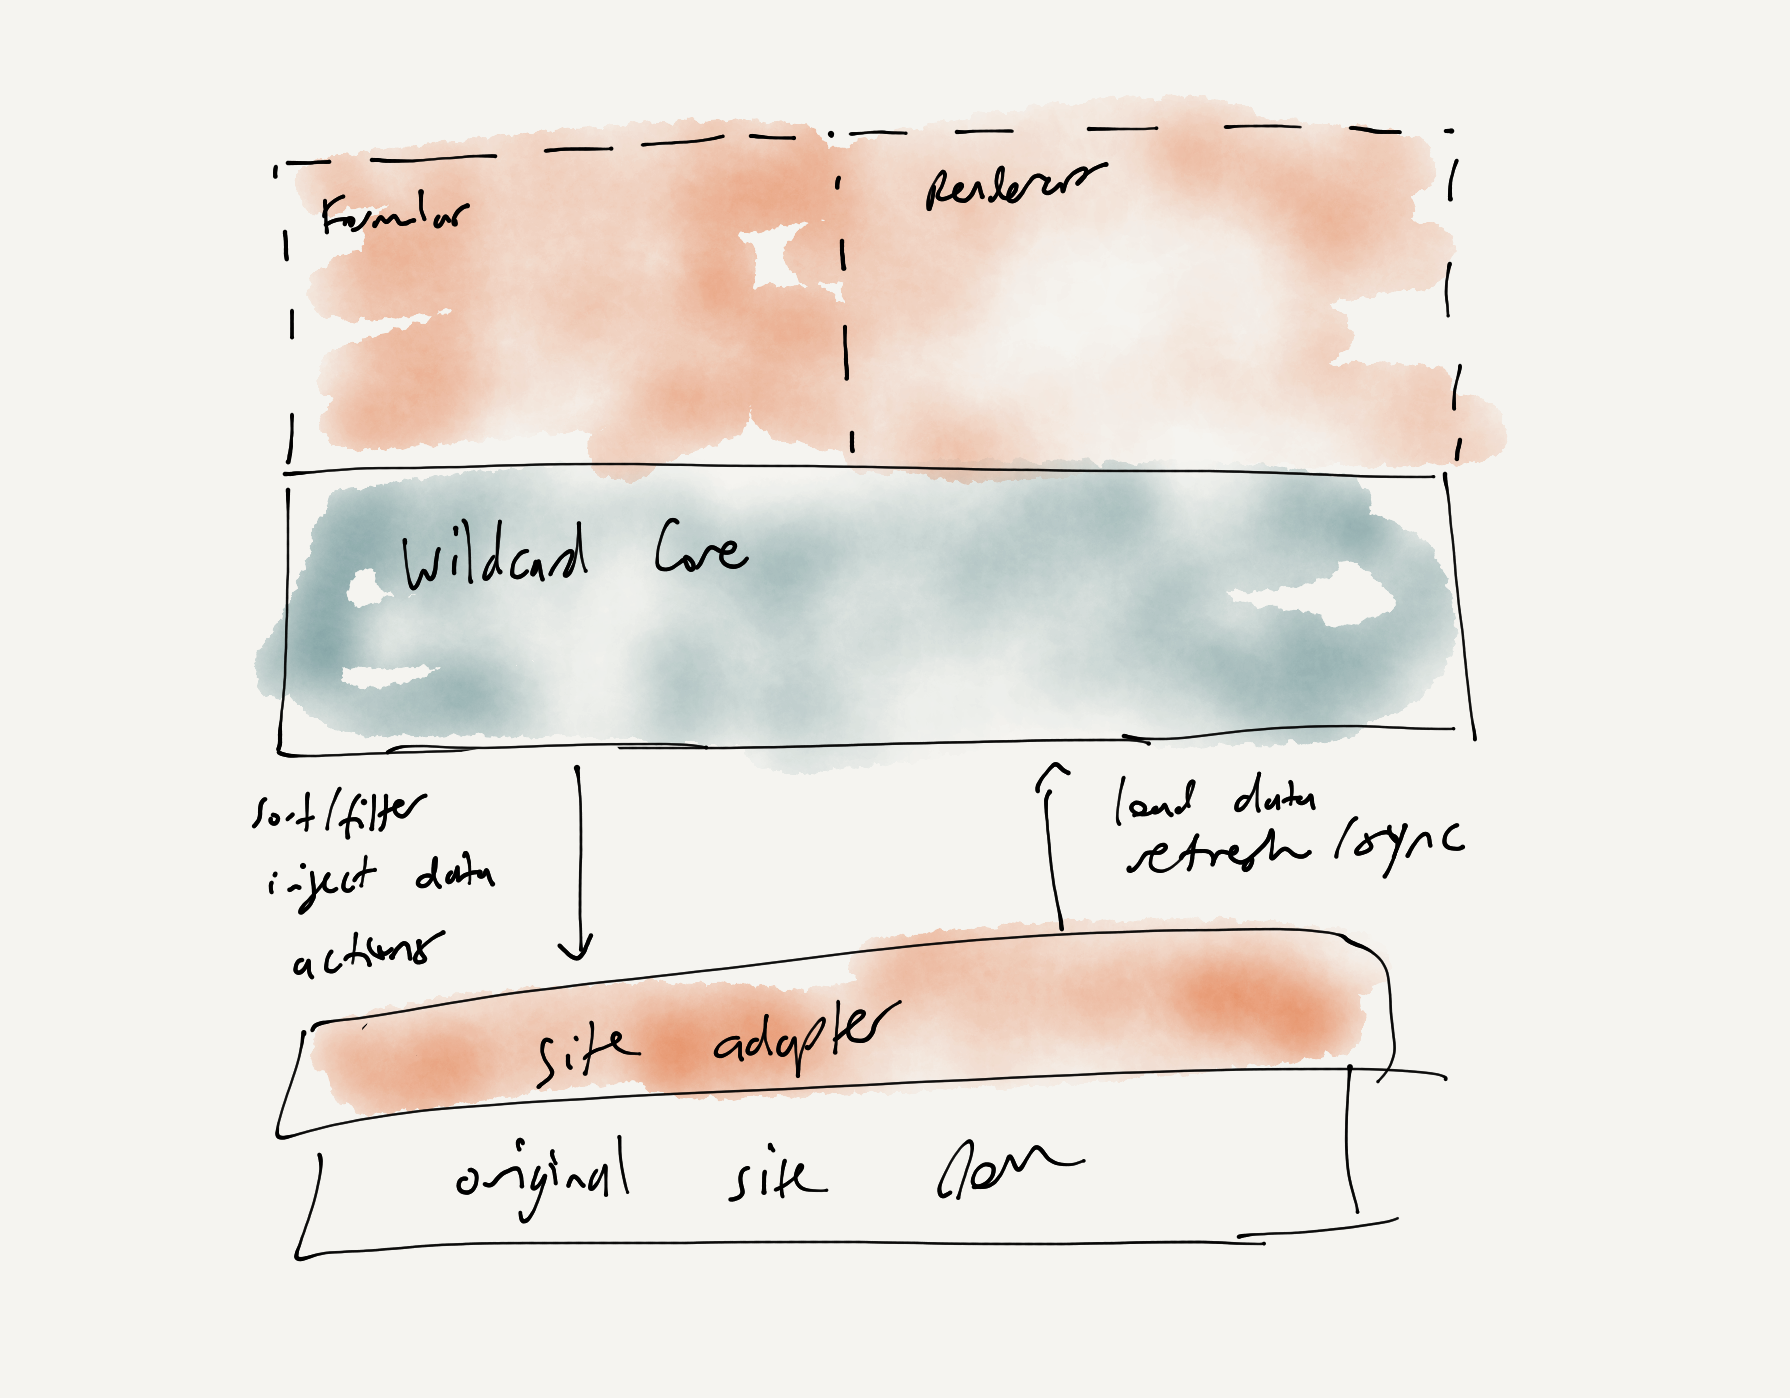
\includegraphics{media/architecture.png}
\caption{The architecture of the Wildcard system}
\end{figure}

Wildcard is written in Typescript, and is injected into pages using the
\href{https://www.tampermonkey.net/}{Tampermonkey} userscript manager
(although in the future we plan to deploy it as a standalone browser
extension.)

In order to maximize extensibility, Wildcard is implemented as a small
core program along with several types of plugins: site adapters,
formulas, and cell renderers/editors. The core contains functionality
for displaying the data table and handling user interactions, and the
table implementation is currently built on the
\href{https://handsontable.com/}{Handsontable} Javascript library to
enable rapid prototyping.

Site adapters\ldots.

Formula functions\ldots{}

Cell viewers\ldots{}

\begin{itemize}
\tightlist
\item
  Extension points

  \begin{itemize}
  \tightlist
  \item
    site adapters

    \begin{itemize}
    \tightlist
    \item
      show a snippet of adapter code
    \item
      discuss how easy it is for programmers to make adapters
    \item
      discuss possible future automation of adapter creation
    \item
      Mention the technique of scraping data from AJAX requests
    \end{itemize}
  \item
    formula functions
  \item
    cell viewer/editors
  \end{itemize}
\item
  future implementation goals

  \begin{itemize}
  \tightlist
  \item
    make it easy for programmers to add adapters + plugins, and
    distribute them to users. (Currently all adapters + plugins are part
    of the main Wildcard codebase)
  \end{itemize}
\end{itemize}

\hypertarget{design-principles}{%
\section{Design principles}\label{design-principles}}

The design of Wildcard is grounded in several principles, informed by
prior work and our own experimentation. We hope you find these
principles helpful not only for understanding our prototype, but also
for designing other systems for end user programming.

\emph{Todo: add diagrams illustrating principles}

\hypertarget{decouple-ui-from-data}{%
\subsection{Decouple UI from data}\label{decouple-ui-from-data}}

Most software does not allow users to choose their own UI elements, even
for common data types. If a website provides a datepicker widget, you
have no ability to provide your own replacement datepicker, with your
preferred design or with privileged access to your private calendar
data. This forces users to learn many different interfaces of varying
quality for similar tasks. Some websites have APIs to allow users to
access the data underlying the UI, but in addition to requiring
programming, these are heavyweight tools more fit for batch exports or
building entire new clients than for casual UI modification.

In Wildcard, a user gets access to a view of the underlying data in the
page, and can choose their own interfaces to view and modify the data.
The Expedia datepicker demo showed one example of how this can be
useful, but we also envision creating other widgets for visualizing and
editing data. Some examples would be showing geographic data in a custom
map that includes the user's own annotations, or editing a blog post in
a rich text editor of the user's choice.

One benefit of decoupling data from interfaces is improved UI quality.
When UI widgets can compete on their merits rather than based on network
effects from the data they have access to, it creates much stronger
competition at the interface level. For example, there is competition
among email clients (which consume an open protocol), but not among
Facebook or Twitter clients. This benefit relates to the SOLID project
led by Tim Berners-Lee \autocite{berners-lee2018}, which envisions
user-controlled data as a mechanism for decoupling data from interfaces,
e.g.~giving users a choice of which client to use to consume a given
social media feed. Wildcard has overlapping goals with SOLID, but does
not require decentralized user control of data---the data can remain on
a centralized server, as long as the interface can be tweaked by end
users.

Another benefit of decoupling data from UI is that it becomes possible
to use the same consistent interface across many applications. For
example, many programmers become deeply familiar with one text editor
and use it for many different kinds of tasks, even as an interactive
input mechanism in the shell (e.g.~for editing git commit messages). The
ability to generically reuse the text editor in many contexts makes it
worth investing time in mastering the tool. Beaudouin-Lafon and Mackay
refer to this ability to use a UI tool in many contexts as
\emph{polymorphic} interaction \autocite{beaudouin-lafon2000}, noting
that it is a useful technique for keeping interfaces simple while
increasing their power. diSessa also \autocite{disessa2000} notes that
there is a connection between polymorphism and the idea of literacy in a
medium: textual literacy rests on a single rich medium of writing which
can be adapted to many different genres and uses.

\emph{Note: Maybe could relate this section to Concept Reuse?}

\hypertarget{expose-structure}{%
\subsection{Expose structure}\label{expose-structure}}

In \emph{Changing Minds} \autocite{disessa2000}, Andrea diSessa
critiques the design of modern software with a story about a
hypothetical ``nightmare bike.'' Each gear on the nightmare bike is
labeled not with a number, but with an icon describing its intended use:
smooth pavement uphill, smooth pavement downhill, gravel, etc. This
might seem more ``user-friendly'' than numbered gears, but in fact, it
makes it harder to operate the bike. A numerical sequence allows the
user to develop intuition for the structure of the system, but isolated
modes provide a superficial understanding with no grounding in
structure. This understanding might be sufficient for the most common
cases but breaks down in unfamiliar situations. If someone needs to go
uphill on gravel, do they need to try every mode at random?

Many modern software designs fall into this trap, teaching users to use
isolated modes rather than coherent structure, and the problem gets far
worse when operating across multiple applications. Unlike the UNIX
philosophy of small tools interoperating through shared abstractions, in
modern computing each application is in its own silo of data and
functionality.

Wildcard helps people understand and modify the behavior of applications
through the lens of a consistent abstraction: a data table. This
abstraction strikes a balance between being both simple and generic. A
data table is simpler than the DOM tree that describes the details of
the UI, but is also generic enough to describe the essence of many
different kinds of applications.

Creating a structured abstraction to represent a web page is a
deliberate choice, and is not the only way to enable users to modify
websites without directly accessing the DOM. Systems like Chickenfoot
\autocite{bolin2005} and CoScripter \autocite{leshed2008} allow users to
create scripts in an informal language and then perform fuzzy pattern
matching to find elements in the DOM. For example, to find a button
after a textbox in Chickenfoot, the user could type
\texttt{click(find(“button\ just\ after\ textbox”))}. These designs
allow for expressing a wide range of operations, but they don't
explicitly indicate what operations are possible---the user can only see
the original page and imagine the possibilities. In contrast, Wildcard
provides affordances that clearly suggest the availability of certain
actions (e.g.~sorting, editing a cell, adding a column with a derived
value), especially to users who are familiar with spreadsheets. In
addition to giving users more certainty about whether a modification is
possible, these affordances might give users new ideas for things to
try. Just as graphical interfaces better communicate the space of
possible actions than command line interfaces, Wildcard aims to clearly
communicate the space of possible modifications.

\hypertarget{direct-manipulation-of-an-alternate-representation}{%
\subsection{Direct manipulation of an alternate
representation}\label{direct-manipulation-of-an-alternate-representation}}

In Wildcard, users manipulate an alternate representation of a web page.
The interaction with the data table is direct like using a spreadsheet,
but the interaction with the page is indirectly mediated through the
table.

We considered other approaches where the user would interact more
directly with the original UI, e.g.~injecting sort controls into the
page, but decided that the table view had advantages that justified the
cost of adding a layer of indirection:

\begin{itemize}
\tightlist
\item
  \emph{Consistency}: Even across different websites, the table view
  always has the same layout, making it easier to learn to use.
\item
  \emph{Affordances}: The table view suggests possible actions like
  adding a new column, which are challenging to suggest in the context
  of the original page.
\item
  \emph{Blank slate for UI}: When a custom UI element is used to
  manipulate a cell in the data table, there are no conflicts with the
  existing interface of the site.
\end{itemize}

The main challenge of making this design successful is maintaining a
close mapping in the user's mind between the new representation and the
original page (\emph{note: cite Norman? Cognitive Dimensions `closeness
of mapping'?}). Wildcard provides live visual cues as the user navigates
the data table, similar to the highlighting provided by browser
developer tools to indicate the mapping between HTML and the original
page. In practice in our own usage, we have found that this live
highlighting is sufficient to make it clear how the two representations
map to each other.

\hypertarget{encourage-casual-tweaking}{%
\subsection{Encourage casual tweaking}\label{encourage-casual-tweaking}}

\begin{longtable}[]{@{}lll@{}}
\toprule
\endhead
& \emph{Casual} & \emph{Not casual}\tabularnewline
\emph{End user friendly} & \textbf{Wildcard} & IFTTT\tabularnewline
\emph{Requires programming} & browser dev tools & editing open source
desktop applications\tabularnewline
\bottomrule
\end{longtable}

We can evaluate a system for modifying software along two dimensions.
First, the technical capability required of the user: is programming
knowledge needed? Second, the level of effort required: how far out of
their way the user must go to make a change? Can they casually make a
small change, or do they need to make a larger project out of it? These
dimensions are not orthogonal, but they are distinct. For example,
setting up a workflow trigger in an end user programming system like
\href{https://ifttt.com/}{IFTTT} does not require much technical skill,
but it does require leaving the user's normal software and entering a
separate environment. On the other hand, running a Javascript snippet in
the browser console requires programming skills, but can be done
immediately and casually in the flow of using a website.

In addition to requiring no programming skills, Wildcard also aims to
support frequent, small modifications. The Wildcard table appears in the
course of normal web browsing, to ensure that the tools for modification
are close at hand while using the original software. Ink and Switch
refers to this property as having an ``in-place toolchain''
\autocite{inkandswitch2019}.

We also try to make simple changes possible with particularly low
effort, like being able to sort a table in a single click. This property
is inspired by spreadsheets, which can be useful even to someone who has
learned only a small part of their functionality. In contrast, many
traditional programming systems require someone to learn many complex
concepts just to perform a simple task (e.g., needing to learn what
\texttt{public\ static\ void\ main} means to write a Hello World program
in Java).

\hypertarget{first-party-cooperation-optional}{%
\subsection{First party cooperation
optional}\label{first-party-cooperation-optional}}

The Web is an unusually extensible platform. On many other platforms
(e.g.~smartphone operating systems), software is locked down unless
first-party developers explicitly provide hooks for plugins and
interoperability, but on the Web, all client-side code is available for
browser extensions to modify. Application authors can use practices that
make it easier to modify their apps (e.g.~clean semantic markup), or
more difficult (e.g.~code obfuscation), but the default state is
openness. This gives extensions freedom to modify applications in
creative ways that the original developers did not plan for.

Wildcard takes advantage of this openness, and does not depend on
cooperation from first-party website developers. Any programmer can add
support for any website to Wildcard by building a third party adapter.
This design decision acknowledges the pragmatic need to interoperate
with current websites, but we hope that eventually first party website
developers will build in Wildcard support to their applications, since
this would reduce the burden of maintaining adapters and make Wildcard
plugins more stable.

Implementing the Wildcard adapter API could help developers by allowing
users to fix some of their own issues, particularly idiosyncratic use
cases that the first party developer would never plan to prioritize.
Supporting Wildcard could be straightforward in a typical client-side
application that already has access to a structured version of the data
in the page. And while some developers might hesitate to promote
extensibility in their clients to avoid unwanted changes, the most
common problem of users blocking ads is already ground well trod by
existing browser extensions. There is also precedent for first parties
implementing an official client extension API in response to user
demand: for several years, Google maintained an official extension API
in Gmail for Greasemonkey scripts to use. (Incidentally, since then,
third parties have continued to maintain Gmail extension APIs used by
many Gmail browser extensions \autocite{streak,talwar2019}, illustrating
the value of collaboratively maintaining third party adapters.)

\hypertarget{no-magic}{%
\subsection{No magic}\label{no-magic}}

\begin{itemize}
\tightlist
\item
  an ecosystem of programmers collaboratively building a platform for
  end users
\item
  but still empowering end users to do the creative parts, the final
  glue
\item
  less brittle, less confusing and surprising (maybe Chickenfoot or
  Coscripter had this problem? Find a nugget in those papers to support.
  I remember Helena had something about auto-scraping breaking\ldots{}
  contrast with Gmail.Js stability?)
\item
  still leaves the door open for future automation
\item
  maybe ``first party optional'' can be included here?
\end{itemize}

\hypertarget{related-work}{%
\section{Related work}\label{related-work}}

\emph{Note: a lot of this was already covered above; how to deal with
that?}

\begin{itemize}
\tightlist
\item
  Malleable software: Kay, Webstrates
\item
  Instrumental interaction, polymorphic UI
\item
  Web automation: Chickenfoot, CoScripter
\item
  Wrapper induction: Thresher, Helena
\item
  Personal data ownership: SOLID
\item
  Extension helper libraries, e.g.~Gmail.js.
\item
  Doctorow:
  \href{https://www.eff.org/deeplinks/2019/10/adversarial-interoperability/}{adversarial
  interoperability}
\item
  Marmite
\end{itemize}

\hypertarget{future-work}{%
\section{Future work}\label{future-work}}

\begin{itemize}
\tightlist
\item
  limitations / future ideas

  \begin{itemize}
  \tightlist
  \item
    the spreadsheet language is very primitive, can we make it more
    expressive? what are the exact semantics of fetching data from APIs?
    What about making API requests that do mutation, not just fetching
    data?
  \item
    only works when the user is browsing. Should we explore triggers,
    scheduled scraping?
  \item
    only has spreadsheet-style functional transformations. Should we
    explore imperative workflows? Injecting buttons into pages that do
    things? (Eg, imagine a ``save to google maps'' button that you can
    inject into a page)
  \item
    limited options for how to style injected content, could explore
    styling (eg, maybe you can restyle a table cell and the styling is
    reflected when it's injected into the page?)
  \item
    how much do adapters generalize to many sites? We've built X
    adapters but need to make more
  \item
    page boundaries, eg scraping multi page results
  \item
    how do people save scripts and share them with each other? TBD
  \item
    nested data? lean on SIEUFERD?
  \item
    reduce the number of primitives?
  \end{itemize}
\item
  still in early development; note the beta release plan (tentative:
  target public beta availability at the workshop in March?)
\item
  Could explore automated wrapper induction, building on prior work
\item
  Want to get more real usage of the tool and run usability studies
\item
  Include a link to sign up for future updates
\end{itemize}

\acks
\printbibliography

\end{document}

% Local Variables:
% TeX-engine: luatex
% End:
